\documentclass[10pt]{article}

\usepackage[margin=1in]{geometry}
\usepackage{microtype}
\usepackage{amsmath,amssymb}
\usepackage{booktabs}
\usepackage{graphicx}
\usepackage{subcaption}
\usepackage{xcolor}
\usepackage{tikz}
\usetikzlibrary{arrows.meta,positioning,calc}
\usepackage{algorithm}
\usepackage{algpseudocode}
\usepackage{listings}
\usepackage{caption}
\usepackage{enumitem}
\usepackage{float}
\usepackage{url}
\usepackage{natbib}
\usepackage{hyperref}

\setlength{\textfloatsep}{10pt plus 2pt minus 4pt}
\setlength{\floatsep}{8pt plus 2pt minus 2pt}
\setlength{\intextsep}{8pt plus 2pt minus 2pt}
\setlength{\abovecaptionskip}{4pt}
\setlength{\belowcaptionskip}{2pt}
\setlist{itemsep=1pt, topsep=3pt, parsep=0pt}

\hypersetup{
  colorlinks=true,
  linkcolor=black,
  citecolor=blue!50!black,
  urlcolor=blue!50!black
}

\lstset{
  basicstyle=\ttfamily\footnotesize,
  breaklines=true,
  columns=fullflexible,
  frame=single,
  framesep=4pt,
  xleftmargin=6pt,
  xrightmargin=6pt,
  aboveskip=8pt,
  belowskip=8pt
}

\newcommand{\Scenic}{\textsc{Scenic}}

\title{Scenario Generation for Asteroid Landing:\\
A \Scenic{} Interface to Basilisk}
\author{Mustafa Ajmal}
\date{August 2026}

\begin{document}
\maketitle

\begin{abstract}
Autonomous asteroid landing is hard to evaluate because the environment is itself uncertain: body shape, surface relief, and approach geometry all vary from encounter to encounter.
This project adds a \Scenic{} simulator interface to Basilisk/MuJoCo so that those variations can be written as probabilistic programs rather than ad-hoc Python resets.
A three-stage curriculum (smooth sphere, random ellipsoid, bumpy procedural rock) drives a fixed scripted soft-brake policy and, separately, a short PPO training loop.
On twelve Scenic-native episodes per stage, the same controller reaches a $3.5\,\mathrm{m/s}$ near-surface gate on every sphere and ellipsoid sample, never meets a stricter $2.8\,\mathrm{m/s}$ ``soft'' gate on those bodies, and succeeds on only two thirds of bumpy rocks---but those successes \emph{are} soft.
The result is a concrete map of when a lander policy works, which is the point of putting Scenic in front of a space-domain simulator.
Short PPO runs do not yet beat the scripted baseline; they mainly show that the Gym path can consume Scenic scenes, and that a few thousand steps is not enough curriculum.
\end{abstract}

\section{Context and Motivation}
\label{sec:intro}

Recent small-body missions have made it clear that ``the asteroid'' is not a single environment.
Hayabusa imaged Itokawa as a rubble pile with a global dichotomy of rough and smooth terrain~\citep{fujiwara2006itokawa}; Hayabusa2 found Ryugu to be a spinning-top rubble pile~\citep{watanabe2019ryugu}; OSIRIS-REx had to pick a site on Bennu among boulders, craters, and poorly constrained local slopes~\citep{lauretta2017osiris}.
Guidance, navigation, and control (GNC) for a lander is therefore a \emph{distributional} problem: the same controller will be asked to work on many shapes, many approach states, and many local surface geometries.

High-fidelity astrodynamics tools already exist.
Basilisk is a modular simulation framework used for spacecraft GNC, with a MuJoCo-backed rigid-body scene, Vizard visualization, and a message-passing architecture for sensors and actuators~\citep{kenneally2020basilisk,basiliskdocs,todorov2012mujoco}.
What those tools do not provide is a compact language for saying ``sample an elongated rock with craters, place a craft on a random inbound trajectory that still faces the body, and reject scenes that start too close.''
That is exactly the niche of Scenic, a probabilistic programming language for cyber-physical scenarios~\citep{fremont2019scenic,fremont2022scenic,vin2023scenic3}.
Scenic has been used extensively with driving simulators such as CARLA and Webots~\citep{dosovitskiy2017carla,michel2004webots,scenicdocs}, but not with Basilisk.

The scientific and engineering interest of the project is therefore dual.
For space autonomy, a scenario layer makes it possible to \emph{stress-test} a lander against a designed distribution of rocks and approaches, instead of a handful of hand-built initial conditions.
For Scenic, a Basilisk backend is a case study that the language is not tied to driving: the same generate/simulate/record loop can drive a spacecraft if the world model and actions are defined carefully.

This report describes that interface, the asteroid curriculum built on top of it, the challenges in making Scenic's sampled rock the same rock Basilisk integrates, and the empirical picture that results.

\section{Problem Definition}
\label{sec:problem}

The problem is: \emph{use Scenic to generate asteroid-landing scenarios, run them in Basilisk, and measure when a lander policy succeeds or fails.}

Concretely, a scene comprises
\begin{enumerate}[leftmargin=1.4em,itemsep=2pt]
  \item a rigid asteroid whose shape is drawn from a designed family (sphere, ellipsoid, or noisy rock with bumps/craters/ridges);
  \item a spacecraft with sampled inertial position, velocity, and attitude;
  \item hard constraints (Scenic \texttt{require}) that keep the craft in a plausible approach envelope;
  \item a closed-loop controller that issues a scalar throttle on the body $+z$ thruster, optionally with a pointing command.
\end{enumerate}
Dynamics live in Basilisk/MuJoCo.
Scenic owns sampling, behaviors, termination, and instrumentation.

Success is not a single binary.
Following the landing literature's emphasis on both proximity and impact speed~\citep{scheeres2012orbital}, three anytime gates are scored on the recorded altitude/speed traces:
\begin{itemize}[leftmargin=1.4em,itemsep=2pt]
  \item \textbf{Contact:} mesh-radar altitude $h \in [0.3, 8]\,\mathrm{m}$ at some time.
  \item \textbf{Reach} (primary ``safe'' metric): contact and inertial speed $v \le 3.5\,\mathrm{m/s}$.
  \item \textbf{Soft:} contact and $v \le 2.8\,\mathrm{m/s}$.
\end{itemize}
The gates are intentionally permissive relative to a flight-like touchdown spec.
The goal of this case study is to \emph{distinguish} easy from hard Scenic worlds, not to certify a flight controller.

Two evaluation paths address the same question from different sides:
\begin{description}[leftmargin=1.1em,style=nextline]
  \item[Path A --- Scenic-native.]
    A scripted Scenic behavior runs inside \texttt{simulate()}.
    Mesh-radar altitude is the live \texttt{ego.altitude} the behavior reads.
  \item[Path B --- Gym curriculum.]
    The same \texttt{.scenic} files reset a Gymnasium environment~\citep{towers2024gymnasium}.
    A Python scripted policy and a short PPO policy~\citep{schulman2017ppo,raffin2021sb3} are compared for transfer across stages.
\end{description}
Camera-based site selection, vision-language models, multi-thruster allocation, and reaction wheels are explicitly out of scope.

\section{Related Work}
\label{sec:related}

\paragraph{Scenic.}
Scenic~1 introduced a probabilistic scene language with geometric specifiers, hard requirements, and rejection sampling~\citep{fremont2019scenic}.
Scenic~2 added dynamic agents, behaviors, and a simulator API~\citep{fremont2022scenic}.
Scenic~3 extended the spatial model to 3D meshes and occupancy~\citep{vin2023scenic3}.
Official backends exist for CARLA, Webots, GTA~V, LGSVL, a Newtonian physics engine, and others~\citep{scenicdocs}.
The recommended path for a new backend is a \texttt{Simulator}/\texttt{Simulation} pair plus a world-model library~\citep{scenicdocs}.
This project follows that recipe for Basilisk.

\paragraph{Space simulation and landing GNC.}
Basilisk provides flight-like messaging, integrators, and visualization~\citep{kenneally2020basilisk}.
MuJoCo supplies the contact-capable rigid-body scene~\citep{todorov2012mujoco}.
Modified Rodrigues parameters (MRPs) are the native attitude representation~\citep{schaub1996mrp}.
Asteroid proximity operations are classically treated in a body-fixed frame with irregular gravity~\citep{scheeres2012orbital}.
This demo uses a constant inertial force for a first closed loop, with a central-gravity option left in the backend.

\paragraph{Randomized worlds and curricula.}
Domain randomization treats simulator parameters as a distribution so that a policy cannot overfit one mesh~\citep{tobin2017domain}.
Curriculum learning presents tasks in an easy-to-hard order~\citep{bengio2009curriculum}.
Both ideas appear here, but as Scenic programs (distributions plus \texttt{require}) rather than unnamed Python noise on a reset.

\paragraph{Prior code.}
The dynamics, Gym environment, scripted/PPO policies, and Vizard plumbing live in the sibling package \texttt{asteroid-rl-demo}~\citep{asteroidrldemo}.
Before this project, that stack used either a flat pad or a stock Itokawa heightmap and ``Scenic-like'' Gaussian starts---randomization without the Scenic compiler.
The contribution here is the real Scenic world model, the procedural mesh that Scenic samples, and the closed loop that keeps that mesh consistent from language to physics.

\section{Approach}
\label{sec:approach}

\subsection{System architecture}

Figure~\ref{fig:arch} is the runtime.
A \texttt{.scenic} file is compiled with \texttt{scenarioFromFile}; each \texttt{generate()} draw produces a \texttt{Scene}.
\texttt{BasiliskSimulation.setup} walks the scene objects, builds either a stock Itokawa scene or a fresh procedural MuJoCo XML, and soft-resets the hub to the sampled pose and velocity.
Each control step, Scenic behaviors emit actions; the backend flushes throttle and pointing into Basilisk messages and advances the integrator by $\Delta t = 0.25\,\mathrm{s}$.
Dynamic properties (\texttt{position}, \texttt{velocity}, \texttt{altitude}, \texttt{throttle}) are read back so that closed-loop Scenic code and \texttt{record} statements see live physics, not the initial sample.

\begin{figure}[t]
\centering
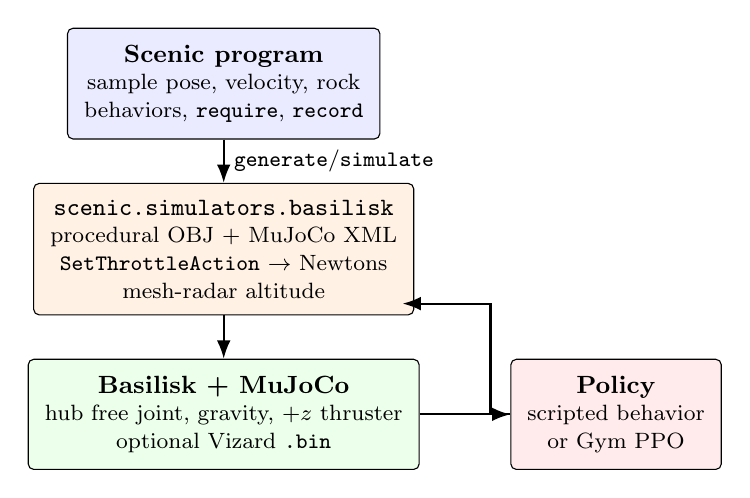
\begin{tikzpicture}[
  font=\small,
  box/.style={draw, rounded corners=2pt, align=center, inner sep=6pt, fill=black!3},
  arr/.style={-{Latex}, thick}
]
\node[box, fill=blue!8] (sc) {\textbf{Scenic program}\\[-1pt]
{\footnotesize sample pose, velocity, rock}\\[-1pt]
{\footnotesize behaviors, \texttt{require}, \texttt{record}}};
\node[box, fill=orange!10, below=0.55cm of sc] (if) {\textbf{\texttt{scenic.simulators.basilisk}}\\[-1pt]
{\footnotesize procedural OBJ + MuJoCo XML}\\[-1pt]
{\footnotesize \texttt{SetThrottleAction} $\to$ Newtons}\\[-1pt]
{\footnotesize mesh-radar altitude}};
\node[box, fill=green!8, below=0.55cm of if] (bsk) {\textbf{Basilisk + MuJoCo}\\[-1pt]
{\footnotesize hub free joint, gravity, $+z$ thruster}\\[-1pt]
{\footnotesize optional Vizard \texttt{.bin}}};
\node[box, fill=red!8, right=1.15cm of bsk] (pol) {\textbf{Policy}\\[-1pt]
{\footnotesize scripted behavior}\\[-1pt]
{\footnotesize or Gym PPO}};
\draw[arr] (sc) -- node[right, font=\footnotesize] {\texttt{generate}/\texttt{simulate}} (if);
\draw[arr] (if) -- (bsk);
\draw[arr] (bsk) -- (pol);
\draw[arr] (pol.west) -- ++(-0.25,0) |- ($(if.south east)+(-0.15,0.15)$);
\end{tikzpicture}
\caption{Scenic samples the world and the approach; Basilisk integrates the craft; the policy closes the loop on live altitude and speed.
The same \texttt{.scenic} files feed Path~A (in-process Scenic behaviors) and Path~B (Gym resets).}
\label{fig:arch}
\end{figure}

Ground truth is Cartesian inertial: position $\mathbf{r}$, velocity $\mathbf{v}$, MRP $\boldsymbol{\sigma}_{BN}$, and body rate $\boldsymbol{\omega}_{BN}^{B}$.
There is no latitude/longitude frame.
Peak thrust is $275\,\mathrm{N}$ on a single body $+z$ actuator; pointing aims body $-z$ (boresight) so that a burn is anti-velocity when the craft faces the rock.

\subsection{World model}

The Scenic library \texttt{scenic.simulators.basilisk.model} defines the entities a scenario author actually writes:
\texttt{Spacecraft}, stock \texttt{Asteroid} (Itokawa), \texttt{ProceduralAsteroid}, and terrain kinds \texttt{AsteroidBump}, \texttt{AsteroidCrater}, \texttt{AsteroidRidge}.
A procedural rock is an icosphere scaled to radii $(r_x, r_y, r_z)$, displaced by multi-octave hash noise of amplitude \texttt{noiseAmp}, then folded with Gaussian hills, bowl-plus-rim craters, and anisotropic ridges---the same compositional idea as Scenic's Mars/Webots terrain lists, but on a closed body rather than a heightmap.
Each \texttt{generate()} also samples \texttt{detailSeed}, so fine roughness changes even when the bump count is fixed.

Terrain objects are \emph{not} independent MuJoCo bodies.
They contribute only to mesh generation at build time; otherwise Scenic would treat them as free-floating collision objects, which is the wrong physics for a rock.

\subsection{Mesh-radar altitude}

A spherical-shell ``altitude'' $|\mathbf{r}-\mathbf{r}_{\mathrm{ast}}|-\bar{r}$ is wrong on an ellipsoid, and a flat-pad $z-z_{\mathrm{pad}}$ is wrong on any closed body.
The backend therefore raycasts from the craft toward the asteroid center of mass and returns the first triangle hit (Figure~\ref{fig:ray}).
That quantity is what Scenic behaviors read as \texttt{ego.altitude}, what \texttt{record} writes, and what Path~A gates score.
It is the closest stand-in in this demo for a nadir altimeter; a true Basilisk \texttt{simpleNav} radar module is future work.

\begin{figure}[t]
\centering
\begin{subfigure}[t]{0.46\textwidth}
\centering
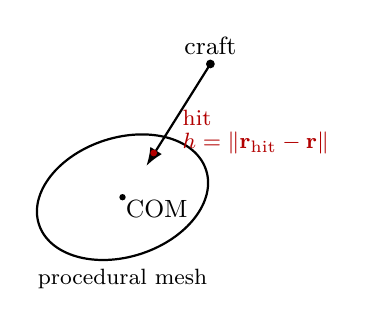
\begin{tikzpicture}[scale=0.72, font=\small]
  \draw[thick, rotate=18] (0,0) ellipse (1.55 and 1.05);
  \fill (0,0) circle (1.6pt) node[below right, inner sep=1pt] {COM};
  \fill (1.55,2.35) circle (2.2pt) node[above] {craft};
  \draw[-{Latex}, thick] (1.55,2.35) -- (0.42,0.55);
  \fill[red!70!black] (0.55,0.78) circle (1.7pt);
  \node[font=\footnotesize, red!70!black, align=left] at (2.35,1.15) {hit\\[-1pt]$h=\|\mathbf{r}_{\mathrm{hit}}-\mathbf{r}\|$};
  \node[font=\footnotesize] at (0,-1.45) {procedural mesh};
\end{tikzpicture}
\caption{Altitude is a raycast along craft$\to$COM, not a spherical shell or pad $z$.}
\label{fig:ray}
\end{subfigure}\hfill
\begin{subfigure}[t]{0.50\textwidth}
\centering
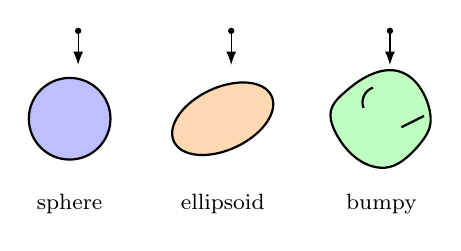
\begin{tikzpicture}[scale=0.72, font=\small]
  \begin{scope}[shift={(0,0)}]
    \draw[thick, fill=blue!25] (0,0) circle (0.72);
    \fill (0.15,1.55) circle (1.6pt);
    \draw[-{Latex}] (0.15,1.55) -- (0.15,0.95);
    \node[below, font=\footnotesize] at (0,-1.15) {sphere};
  \end{scope}
  \begin{scope}[shift={(2.7,0)}]
    \draw[thick, fill=orange!30, rotate=25] (0,0) ellipse (0.95 and 0.55);
    \fill (0.15,1.55) circle (1.6pt);
    \draw[-{Latex}] (0.15,1.55) -- (0.15,0.95);
    \node[below, font=\footnotesize] at (0,-1.15) {ellipsoid};
  \end{scope}
  \begin{scope}[shift={(5.5,0)}]
    \draw[thick, fill=green!25] plot[smooth cycle, tension=0.65]
      coordinates {(0.85,0.15) (0.55,0.7) (0.05,0.85) (-0.55,0.55)
                   (-0.9,0.05) (-0.5,-0.65) (0.15,-0.85) (0.75,-0.35)};
    \draw[thick] (-0.15,0.55) arc (110:200:0.28);
    \draw[thick] (0.35,-0.15) -- (0.75,0.05);
    \fill (0.15,1.55) circle (1.6pt);
    \draw[-{Latex}] (0.15,1.55) -- (0.15,0.95);
    \node[below, font=\footnotesize] at (0,-1.15) {bumpy};
  \end{scope}
\end{tikzpicture}
\caption{Curriculum: sphere, ellipsoid, then noisy rock plus terrain.}
\label{fig:curr}
\end{subfigure}
\end{figure}

\subsection{Curriculum}

Three Scenic programs share a world model and differ only in the distributions they impose (Figure~\ref{fig:curr}):
\begin{description}[leftmargin=1.1em,style=nextline]
  \item[\texttt{sphere.scenic}]
    Radii $45\,\mathrm{m}$ isotropic, zero noise, no terrain.
    Craft $z \in [20,45]\,\mathrm{m}$, small lateral offset and velocity.
  \item[\texttt{ellipsoid.scenic}]
    Independent radii $r_x \in [40,60]$, $r_y \in [30,50]$, $r_z \in [28,45]$, light noise, random body placement.
  \item[\texttt{bumpy.scenic}]
    Wider radii, \texttt{noiseAmp} $\in [1.5, 3.5]$, subdivision 3, twenty bumps, sixteen craters, eight ridges, and a more aggressive inbound velocity box.
\end{description}
All three require the craft--asteroid distance to lie in a window (roughly $120$--$260\,\mathrm{m}$) so that rejection sampling discards degenerate overlaps or escapes.
They terminate at $h < 4\,\mathrm{m}$ or after $60\,\mathrm{s}$.

\subsection{Controllers}

Path~A uses the Scenic behavior in Algorithm~\ref{alg:brake} (bumpy uses slightly earlier/heavier braking: $22\,\mathrm{m}$ / $2.5\,\mathrm{m/s}$ instead of $20\,\mathrm{m}$ / $2.8\,\mathrm{m/s}$).
The policy is memoryless and privileged only in that it sees true mesh-radar altitude and inertial speed---no camera, no site-relative lateral state.

\begin{algorithm}[t]
\caption{Scripted soft-brake behavior (sphere / ellipsoid).}
\label{alg:brake}
\begin{algorithmic}[1]
\Repeat
  \If{$h < 20\,\mathrm{m}$}
    \State point body $-z$ to inertial $-\hat{\mathbf{z}}$; throttle $\leftarrow 1.0$
  \ElsIf{$h < 50\,\mathrm{m}$ \textbf{and} $v > 1.5\,\mathrm{m/s}$}
    \State point nadir; throttle $\leftarrow 0.7$
  \ElsIf{$v > 2.8\,\mathrm{m/s}$}
    \State point nadir; throttle $\leftarrow 0.4$
  \Else
    \State coast (throttle $0$)
  \EndIf
\Until{Scenic terminates the simulation}
\end{algorithmic}
\end{algorithm}

Path~B trains PPO (\texttt{MlpPolicy}, $n_{\mathrm{steps}}=256$, batch $64$, $\mathrm{lr}=3{\times}10^{-4}$) on Gym observations in \texttt{truth} mode (altitude, vertical rate, site distance, speed, previous throttle), with \texttt{auto\_point} aiming the thruster.
Two training regimes were run: $5{,}000$ steps on sphere only, and a progressive $4{,}000$ steps per stage (sphere then ellipsoid then bumpy).
Those budgets are proof-of-life, not a claim about asymptotic RL performance.

\subsection{Instrumentation}

Each scenario records
\[
\texttt{altitude\_m},\; \texttt{speed\_mps},\; \texttt{throttle},\; \texttt{z\_m}
\]
into \texttt{sim.result.records}.
After \texttt{simulate()} returns, Scenic clears dynamic object properties, so the evaluator must score the record dictionary rather than \texttt{ego.altitude} on the Python object.
Per-episode CSVs and optional Vizard \texttt{.bin} files are written for plots and replay.

\section{Challenges}
\label{sec:challenges}

\paragraph{A new Scenic simulator, not a wrapper script.}
Scenic's contract is specific: subclass the simulator and simulation classes, implement the step/action/property hooks, and declare \texttt{[dynamic]} fields in the world model~\citep{scenicdocs}.
A one-shot ``run Basilisk from Python'' script would sample an initial condition but could not run Scenic behaviors against live altitude.
Most of the engineering was making that loop correct, including converting Scenic yaw, pitch, and roll to MRPs~\citep{schaub1996mrp} and body rates back to inertial $\boldsymbol{\omega}$.

\paragraph{The sampled rock must be the integrated rock.}
An early Gym path compiled Scenic only for craft initial conditions and then loaded stock Itokawa.
Policies were then being scored on a body they had not been promised.
The fix is to rebuild the MuJoCo XML from the Scenic mesh on every \texttt{generate()} (\texttt{reuse\_sim=False} in Gym).
Until that gap closed, transfer numbers were not about shape difficulty; they were about two different planets.

\paragraph{Altitude semantics.}
Pad-$z$ altitude made a spherical approach look like a landing on a plane at $z=-30\,\mathrm{m}$.
A mean-radius shell ignored ridges that a real altimeter would see tens of meters early.
Raycasting toward COM is still an approximation---it is not a body-axis boresight altimeter, and it can glance a ridge while the velocity vector is elsewhere---but it is the quantity the PI asked for and the one the scripted policy actually uses.

\paragraph{Windows visualization.}
Live ZeroMQ streaming to Vizard is fragile on Windows (bind timeouts, \texttt{epoll} noise).
The practical mode is \texttt{viz\_mode='file'}: write a \texttt{.bin} and replay with \texttt{-loadFile}.
That is a tooling constraint, not a science one, but it blocked ``just look at the rock'' debugging until file mode was wired through Scenic params.

\paragraph{Scoring too strictly hides the curriculum.}
A first sweep used a tighter safe-landing gate and reported $0\%$ success on sphere and ellipsoid even though every trajectory arrived at $\sim\!3.1\,\mathrm{m/s}$ and $\sim\!3.5\,\mathrm{m}$ altitude.
The dual-metric gates in Section~\ref{sec:problem} were introduced so that ``always reaches, never soft'' on smooth bodies and ``sometimes fails, but softly when it works'' on bumpy bodies could both be seen.
Choosing gates is part of the experimental design; it is also a place where a writeup can accidentally manufacture a null result.

\paragraph{The two scripted policies are not the same.}
Path~B's baseline is the Python controller inside \texttt{asteroid-rl-demo}, not Algorithm~\ref{alg:brake}.
Combined with Gym's terminal (not anytime) \texttt{safe\_landing} and a $120\,\mathrm{s}$ timeout, ellipsoid scripted episodes often coast out at tens to hundreds of meters.
Path~A and Path~B therefore answer related but not identical questions; they should not be averaged together.

\paragraph{Short PPO is not a curriculum result.}
Four to five thousand steps is enough to confirm that Scenic scenes are valid Gym resets.
It is not enough to learn a throttle law that dominates a tuned script, and a progressive run of $4\mathrm{k}$ steps per stage is a recipe for forgetting the first stage.
Those negative results are reported in Section~\ref{sec:results} rather than hidden.

\section{Results}
\label{sec:results}

\subsection{Path A: fixed policy, Scenic worlds}

Table~\ref{tab:patha} and Figure~\ref{fig:ratesa} summarize twelve episodes per stage (seed $0$ plus offsets), all with mesh-raycast altitude.

\begin{table}[t]
\centering
\caption{Path~A, 12 episodes/stage.
Reach is the primary safe metric ($h\in[0.3,8]\,\mathrm{m}$, $v\le 3.5\,\mathrm{m/s}$, anytime).}
\label{tab:patha}
\begin{tabular}{@{}lccccc@{}}
\toprule
Stage & Contact & Reach & Soft & Mean $v_f$ (m/s) & Mean $\min h$ (m) \\
\midrule
Sphere     & 100\% & 100\% & 0\%  & 3.10 & 3.56 \\
Ellipsoid  & 100\% & 100\% & 0\%  & 3.17 & 3.67 \\
Bumpy      & 67\%  & 67\%  & 67\% & 1.75 & 6.40 \\
\bottomrule
\end{tabular}
\end{table}

\begin{figure}[t]
\centering
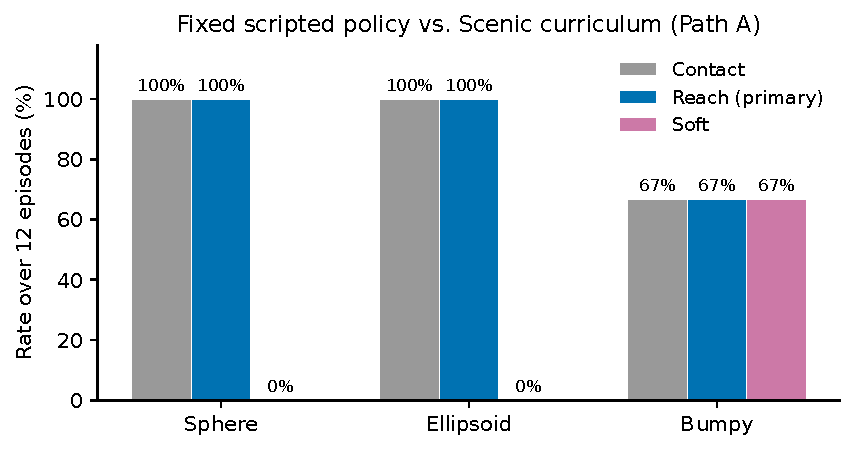
\includegraphics[width=0.72\textwidth]{figures/rates_path_a.pdf}
\caption{The scripted policy is not uniformly ``good'' or ``bad'': smooth bodies always reach and never meet the soft gate; bumpy bodies fail a third of the time and are soft when they succeed.}
\label{fig:ratesa}
\end{figure}

Two patterns matter more than the headline percentages.

First, \textbf{smooth bodies are a speed problem, not a geometry problem.}
Every sphere and ellipsoid episode enters the altitude band, and every one does so between roughly $2.9$ and $3.4\,\mathrm{m/s}$---under the reach gate, over the soft gate (Figure~\ref{fig:scatter}).
The scripted law of Algorithm~\ref{alg:brake} is a late, coarse brake.
On a predictable sphere that is enough to arrive, not enough to arrive gently.

Second, \textbf{bumpy bodies are a geometry problem that also changes speed.}
Failures are not high-speed impacts.
They are episodes whose mesh-radar altitude never drops through $8\,\mathrm{m}$: the craft hangs on full throttle above local relief, or the raycast rides a ridge (dashed curve in Figure~\ref{fig:traj}, open triangles in Figure~\ref{fig:scatter}).
When the bumpy policy \emph{does} enter the band, terminal speed is much lower (median near $1.3\,\mathrm{m/s}$) because the bumpy behavior brakes earlier.
The same family of controller, pointed at a harder Scenic distribution, produces both the only soft landings and the only misses.

\begin{figure}[t]
\centering
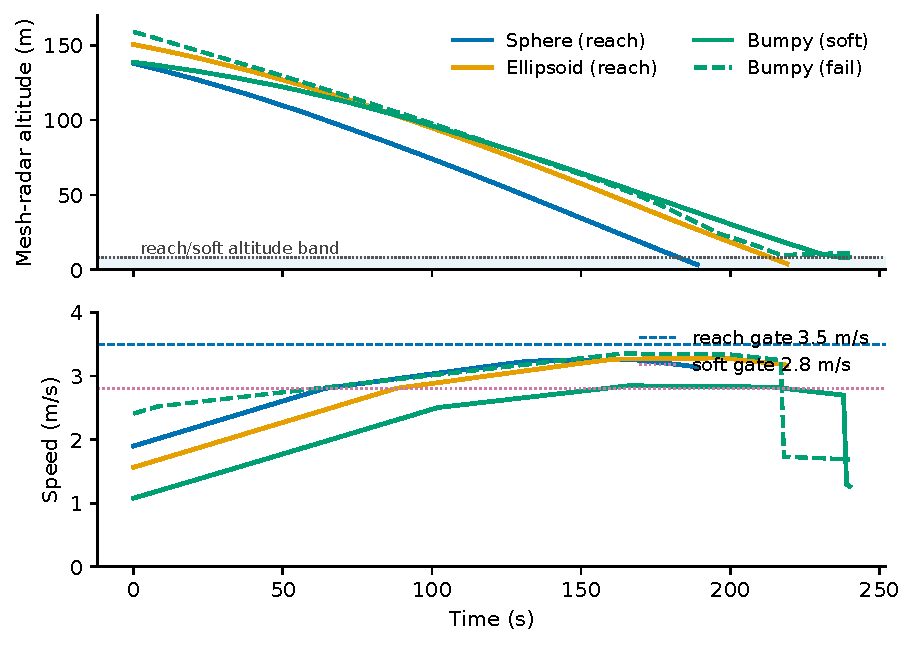
\includegraphics[width=0.82\textwidth]{figures/trajectories.pdf}
\caption{Representative altitude and speed traces.
Sphere and ellipsoid (solid blue/orange) descend into the band just above $3\,\mathrm{m/s}$.
Bumpy success (solid green) brakes into the soft gate; bumpy failure (dashed) levels off near $11\,\mathrm{m}$ on full throttle.}
\label{fig:traj}
\end{figure}

\begin{figure}[t]
\centering
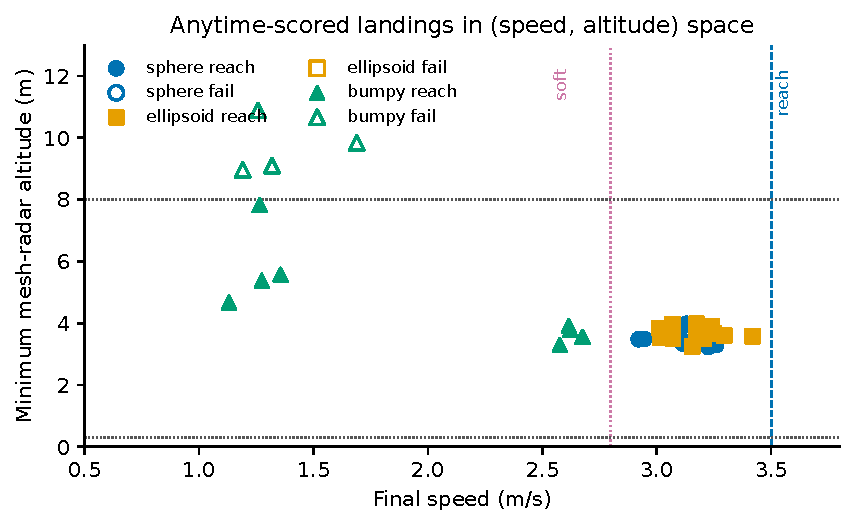
\includegraphics[width=0.72\textwidth]{figures/scatter_gates.pdf}
\caption{Each point is one episode's $(\text{final speed},\,\min h)$.
Filled markers meet reach; open markers do not.
Sphere/ellipsoid cluster just left of $3.5\,\mathrm{m/s}$ and below $8\,\mathrm{m}$.
Bumpy successes sit left of $2.8\,\mathrm{m/s}$; bumpy failures sit above the altitude band at low speed.}
\label{fig:scatter}
\end{figure}

A five-episode subset with Vizard recordings (seeds $0$--$4$) reproduces the same structure: sphere and ellipsoid $5/5$ reach and $0/5$ soft; bumpy $4/5$ reach and $4/5$ soft.
The missing bumpy episode is seed~1, whose altitude bottoms out at $9.8\,\mathrm{m}$.

These numbers are small-$N$ by design---the point is a distinguishable curriculum, not a confidence interval on a $67\%$ rate.
What they show is that Scenic is doing the job asked of it: one controller, three named distributions, a non-trivial success/failure split that tracks the rock, not the random seed of the integrator.

\subsection{Path B: Gym + short PPO}

Figure~\ref{fig:ratesb} reports four eval episodes per cell after (left) $5\mathrm{k}$ PPO steps on sphere only and (right) $4\mathrm{k}$ steps per stage in order.

\begin{figure}[t]
\centering
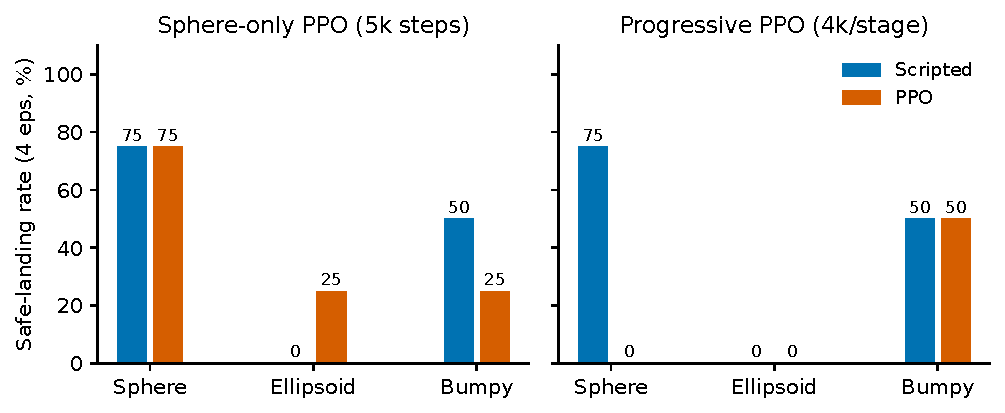
\includegraphics[width=0.92\textwidth]{figures/rates_path_b.pdf}
\caption{Gym safe-landing rates.
Left: a sphere-trained PPO matches scripted on sphere, slightly beats it on ellipsoid, and loses on bumpy.
Right: progressive training forgets the sphere ($0\%$) while matching scripted on bumpy.
$N=4$ per cell; treat as a smoke test, not a ranking of algorithms.}
\label{fig:ratesb}
\end{figure}

The sphere-only PPO matching the scripted $75\%$ on sphere is the optimistic reading: a learned throttle can copy a simple law on the training distribution, and it is not completely incompetent on a new ellipsoid ($1/4$ vs.\ $0/4$).
It does not transfer to bumpy ($1/4$ vs.\ scripted $2/4$).
That is consistent with the Path~A story---shape is the thing that breaks a law tuned on a smooth body---but the sample is too small to say more.

The progressive run is the pessimistic reading, and the more informative one for future work.
After visiting ellipsoid and bumpy, PPO is $0/4$ on the stage it started with.
Catastrophic forgetting under a tiny per-stage budget is the expected failure mode, not a surprise about asteroids.
It does confirm that the plumbing works: each reset really did rebuild a Scenic mesh, or the agent could not have specialized to bumpy at all.

Gym ellipsoid scripted at $0\%$ also illustrates Section~\ref{sec:challenges}: several of those episodes time out at $50$--$200\,\mathrm{m}$ altitude under a \emph{different} scripted law and a terminal gate.
They should not be cited as ``ellipsoids are impossible''; Path~A already shows the opposite for Algorithm~\ref{alg:brake}.

\subsection{What did not work}

A few things failed in ways that are worth keeping in the narrative.
Live Vizard on Windows was not a usable development loop.
Treating terrain features as ordinary Scenic objects with collision produced nonsense physics until they were demoted to mesh displacements.
Flat-pad and spherical-shell altitudes made the curriculum look flatter than the rocks were.
Over-strict scoring made Path~A look like a total failure.
And PPO, at the compute budget used here, did not produce a policy one would prefer to the script.
The interface and the Path~A distinction are the results that stand.

\section{Conclusions and Future Work}
\label{sec:concl}

Scenic can sit in front of Basilisk.
The engineering content of the project is a world model, a procedural mesh compiler, a raycast altimeter, and a \texttt{Simulation} object that honors Scenic's dynamic-agent contract.
The scientific content is a small but readable case study: a named easy$\to$hard family of landing worlds that splits a fixed controller into ``always reaches but never softly,'' versus ``sometimes misses the band, and is soft when it does not.''

That split is what a scenario language is for.
It is more useful, at this stage, than a claim that PPO is better or worse than a script.
The curriculum is specified in a few dozen lines of Scenic, not in an undocumented reset function, and the same files drive both an in-process evaluator and a Gym training loop.

Natural next steps, in roughly increasing ambition:
\begin{enumerate}[leftmargin=1.4em,itemsep=3pt]
  \item \textbf{Longer, stabler learning.}
    Tens of thousands of steps per stage, a frozen encoder or replay from earlier stages, and the \emph{same} scripted law as a Path~A baseline inside Gym.
  \item \textbf{Better sensing.}
    Body-axis altimeter, Basilisk \texttt{simpleNav}, and eventually a camera/VLM site selector---the original longer-horizon stack, now with a scenario layer underneath.
  \item \textbf{Better dynamics.}
    Central gravity, rotating bodies, multi-thruster allocation, and reaction wheels, so that ``hard'' means orbital mechanics rather than only mesh relief.
  \item \textbf{Scenic as a falsifier.}
    Once a stronger policy exists, use Scenic requirements to search for the approach that breaks it (the classical Scenic use-case in driving~\citep{fremont2022scenic}), rather than only to sample a fixed curriculum.
  \item \textbf{Real shapes in the language.}
    Promote the Itokawa mesh from a stock backend option to a Scenic object with sampled pose, so that ``this specific rubble pile, random inbound state'' is a one-line scenario.
\end{enumerate}

The lesson I would keep is narrow.
If the environment is the uncertainty, write the environment as a distribution, couple it to the real dynamics, and instrument the quantity the controller actually uses.
Scenic plus Basilisk is one way to do that for asteroid landing; the tables in Section~\ref{sec:results} are evidence that the resulting worlds are not all the same.

\bibliographystyle{plainnat}
\bibliography{references}

\appendix
\section{Scenic curriculum fragment}
\label{app:scenic}

The bumpy stage is representative of how much of the experiment lives in the scenario file rather than in Python.
Radii, noise, terrain counts, inbound state, requirements, records, and the behavior thresholds are all Scenic:

\begin{lstlisting}
asteroid = new ProceduralAsteroid at (Range(-25,25), Range(-25,25),
                                      -150 + Range(-15,15)),
    with radiusX Range(38, 65), with radiusY Range(30, 55),
    with radiusZ Range(28, 50), with subdivisions 3,
    with detailSeed Range(0, 1e9), with noiseAmp Range(1.5, 3.5),
    with terrain ([new AsteroidBump for _ in range(20)]
                + [new AsteroidCrater for _ in range(16)]
                + [new AsteroidRidge for _ in range(8)])

ego = new Spacecraft at (Range(-18,18), Range(-18,18), Range(12,55)),
    with velocity (Range(-0.35,0.35), Range(-0.35,0.35),
                   Range(-2.4,-1.0)),
    facing toward asteroid, with behavior ScriptedSoftBrake

require distance from ego to asteroid > 120
require distance from ego to asteroid < 260
record ego.altitude as altitude_m
record ego.speed as speed_mps
terminate when ego.altitude < 4
terminate after 60 seconds
\end{lstlisting}

\section{Simulation loop (pseudocode)}
\label{app:loop}

\begin{algorithm}[H]
\caption{One Path~A episode.}
\begin{algorithmic}[1]
\State compile scenario; draw $\textit{scene} \leftarrow \texttt{generate}()$
\State build procedural mesh; write MuJoCo XML; set hub $(\mathbf{r},\mathbf{v},\boldsymbol{\sigma})$
\For{$k = 1 \ldots K_{\max}$}
  \State run Scenic behaviors $\to$ pending throttle and pointing
  \State flush controls; integrate Basilisk for $\Delta t$
  \State $h \leftarrow$ mesh raycast$(\mathbf{r} \to \mathbf{r}_{\mathrm{ast}})$; record $(t,h,v,\text{throttle})$
  \If{$h < 4$ \textbf{or} $t \ge 60\,\mathrm{s}$} \textbf{break}
  \EndIf
\EndFor
\State score contact / reach / soft on the recorded series (anytime)
\end{algorithmic}
\end{algorithm}

\section{Reproducing the tables}
\label{app:repro}

From the Scenic checkout, with \texttt{asteroid-rl-demo} as a sibling and its virtualenv active:
\begin{lstlisting}
export ASTEROID_RL_ROOT=../asteroid-rl-demo
export PYTHONPATH=$PWD/src:$ASTEROID_RL_ROOT
python examples/basilisk/run_mvp.py --mode eval --episodes 12 --seed 0
python examples/basilisk/run_mvp.py --mode train \
    --timesteps-per-stage 4000 --eval-episodes 4 --seed 2
\end{lstlisting}
Path~A summaries are \texttt{sweep\_dual.json} under \texttt{outputs/scenic\_policy\_eval}.
Path~B tables live in \texttt{scenic\_curriculum\_v3} (sphere-only) and \texttt{scenic\_curriculum\_mvp} (progressive).
Figures were generated by \texttt{make\_figures.py} in this folder.

\end{document}
